\chapter{Background}\label{sec:back}
\newthought{The main goal of this thesis} is to improve transfemoral amputee
gait robustness and naturalness by applying neuromuscular models of human
locomotion to control prosthesis hardware capable of dynamic locomotion.
Existing approaches to walking control in humanoid robots and prostheses have
largely failed to reach the levels of stability and dynamism required to match
that of an amputee's lost limb. In this \namecref{sec:back}, we will review
these existing approaches, examine their strengths and weaknesses, and motivate
our specific control and design choices.

\Cref{sec:back_walking_review} categorizes approaches to walking control into
four major groups based on their ability to produce dynamic interactions with
the environment (dynamic vs kinematic) and whether they can produce control
commands using only a subset of state (decentralized vs centralized). As
mentioned earlier, only dynamic, decentralized controls address
\cref{chal:dynamic,chal:incomplete_state} of amputee locomotion
(\cref{sec:intro_challenges}) and are thus suitable for prosthesis control.
\Cref{sec:back_bioinspired_pros_control} dives deeper into a subset of dynamic
decentralized control: bioinspired approaches that seek to model the function of
the lost limb and are thus particularly well suited for prosthesis control.
\Cref{sec:back_pros_design} reviews existing mechanical designs of active
prostheses and examines their ability to enable dynamic locomotion. Finally,
\cref{sec:back_stumble_recovery} will discuss previous work towards empowering
prostheses with active trip recovery modes via explicit detection and
classification of stumbles. 

\section{Fundamental Walking Dynamics and
Control}\label{sec:back_walking_review}

Simple point-mass models of walking can help us understand the fundamental
dynamics that control must shape in order to achieve stable locomotion gaits.
The simplest model that reproduces the center of mass trajectory and ground
reaction forces seen during human walking is the bipedal spring mass model
\citep{geyer2006compliant}. This model, illustrated in \cref{fig:ssm_diagram},
simplifies locomotion to a pair of compliant unidirectional springs connected to
a point mass. When initialized with human-like mass and leg length, the model
can generate characteristic features of human locomotion such as sinusoidal
center of mass trajectories, M-shaped vertical ground reaction forces, S-shaped
horizontal ground reaction forces, and the proper sequence of double and single
support. 

\begin{marginfigure}
    \centering
    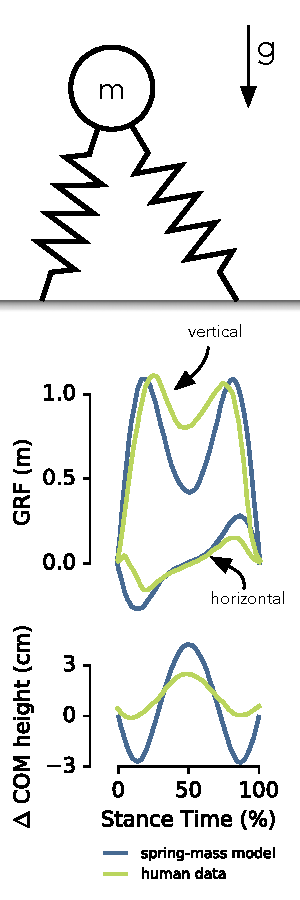
\includegraphics[width=\linewidth]{spring_mass_model_diagram}
    \caption{The bipedal spring mass model captures many fundamental features of
    human walking such as the M-shaped vertical ground reaction profile,
    S-shaped horizontal ground reaction profile and sinusoidal center of mass
    trajectory. Figure adapted from \citet{geyer2006compliant}.}
    \label{fig:ssm_diagram}
\end{marginfigure}

We will look at two paradigms for walking control: centralized approaches that
use full state information and decentralized approaches that use a subset of
state information. Centralized approaches typically utilize a model of the full
system in order to compute control commands that project the full system's
dynamics onto those of the simplified model. Usually, centralized approaches
also place additional constraints on the center of mass (COM) dynamics in order
to facilitate planning and ensure stability. In contrast, decentralized
approaches typically do not explicitly model either the full system or the
fundamental dynamics.  Rather, these approaches use heuristics to generate
motions and forces similar to those of the fundamental model.

\subsection{Centralized Control}\label{sec:back_centralized_control}

\emph{Kinematic centralized control} is one of the oldest forms of locomotion
control. The predominant approach in this category is based on the linear
inverted pendulum model (LIPM) \citep{kajita1991study, kajita20013d}.  This
simplified locomotion model applies additional reductions to the bipedal
spring-mass model, replacing spring legs with ideal prismatic force sources and
constraining the center of mass to move on a plane. The resulting simplified
model features linear COM dynamics with respect to the zero moment point (ZMP).
The ZMP is the point on the ground about the horizontal moments needed to
counteract the total reaction forces on the system is zero. When the ZMP lies
within the support polygon\sidenote{The convex hull of contact points on the
ground} (SP), it is coincident with the center of pressure (COP). On the other
hand, if the ZMP moves beyond the SP, the system will begin to tip over the edge
of the SP. In one dimension, the location of the ZMP is given by, 
\begin{align} 
    x_\textrm{ZMP} = x_\textrm{COM} - \frac{z_\textrm{COM}
        \ddot{x}_\textrm{COM}}{g}. 
    \label{eq:ZMP}
\end{align}
This equation relates the horizontal COM, $x_\textrm{COM}$, dynamics to the
location of the ZMP, $x_\textrm{ZMP}$, given the height of the COM,
$z_\textrm{COM}$, and gravitational acceleration $g$.

Based on this insight, researchers have developed numerous ZMP-trajectory
methods that follow \labelcref{lipm_step_servo} basic steps:
\begin{steps}
    \item Plan a series of foot steps given the terrain and task such that the
    induced sequence of support polygons contains no
    gaps.\label{lipm_step_foot_plan}

    \item Generate a ZMP trajectory that lies within the support polygons.
    Typically, it is desirable that the trajectory maintains its distance from
    the edges of the support polygons in order to provide a margin of
    stability.\label{lipm_step_zmp_traj}

    \item Solve for the COM trajectory given the desired ZMP trajectory. This
    step requires inverting the solution to a differential equation,
    \cref{eq:ZMP}, to solve for $x_\textrm{COM}$. Researchers have proposed
    numerous solutions to this problem including preview control
    \citep{kajita2003biped}, and differential dynamic programming
    \citep{feng2015optimization}, the latter of which can solve for the ZMP and
    COM trajectories simultaneously.\label{lipm_step_com_traj}
    
    \item Use inverse kinematics to calculate joint velocities that track the
    COM trajectory.\label{lipm_step_ik}

    \item Track the desired joint velocities with servo
    controls.\label{lipm_step_servo}
\end{steps}

A large number of robots have successfully employed this general framework to
walk \citep{hirai1998development}, traverse uneven ground
\citep{shimmyo2010biped}, and run \citep{kajita2007zmp}. Moreover, the method
guarantees that for the nominal gait, the COP will remain in the SP, and thus
the system will maintain its stability.

However, there are several key issues to this approach. One issue stems from
\cref{lipm_step_ik,lipm_step_servo} listed above. These steps generate and
precisely follow via servo control a kinematic trajectory of joint angles. When
perturbed by unforeseen external forces, stiff position control in this manner
may generate large reaction forces and thus may move the COP outside of the SP,
resulting in a fall. We can understand the interactions between the leg and the
environment and the leg and robot body through the concepts of impedance and
admittance. The environment and robot body are admittances, objects that take
forces as inputs and move (or not move) in response. As discussed in
\citet{hogan1985impedance}, it is therefore necessary that the leg acts like an
impedance, an object that produces an interaction force in response to the
position imposed on it by the environment and robot body.

\emph{Dynamic centralized control} seeks to control these interaction forces by
directly computing joint torques, instead of using high-gain position control.
Commonly, in this approach the dynamics model of the full
system\sidenote[][-1in]{Where $q$, $\dot{q}$, and $\ddot{q}$ describe the
generalized coordinates, velocities, and accelerations of the system
configuration, $M(q)$ is the mass matrix, $C(q, \dot{q})$ is a matrix of
centripetal and Coriolis force coefficients, $N(q)$ represents the gravitational
forces, $S$ is a selection matrix that assigns joint torques $\tau$ to
coordinates $q$, $J(q)$ is the Jacobian between joint angles and contact points,
and $\lambda$ is a vector of external forces},
\begin{align}
    M(q) \ddot{q} + C(q, \dot{q}) \dot{q} + N(q) = S\tau + J^T(q) \lambda,
    \label{eq:euler_lagrange}
\end{align}
is used as an equality constraint in a \emph{quadratic program} (QP) that
minimizes torques, reaction forces, and deviation from the desired trajectory.
Additionally, the QP can include inequality constraints representing torque
saturations and friction limits \citep{hutter2013hybrid, herzog2014balancing,
saab2013dynamic, wensing2013generation}. Recently, at the DARPA Robotics
Challenge (DRC) several robots used QP-based dynamic centralized approaches to
control humanoid robots through a disaster relief scenario
\citep{feng2015optimization, kuindersma2014efficiently,
englsberger2014trajectory}. 

While the replacing \cref{lipm_step_ik,lipm_step_servo} with a QP-based torque
control can help improve dynamism and compliance, the resulting biped gaits of
these strategies do not resemble human gaits for two reasons: First, the linear
inverted pendulum model does not produce center of mass trajectories or ground
reaction force profiles similar to those seen during human locomotion.  Second,
human gaits do not constrain the ZMP to the support polygon as we spend
significant time on the heel and balls of our feet during stance
\citep{perry1992gait}.

To overcome these issues and produce more human like gaits, recently researchers
have investigated applying dynamic centralized control approaches to enforce
spring-mass model dynamics instead of LIPM dynamics. With this approach,
researchers have developed robust controllers for both walking
\citep{wensing2013generation} and running \citep{martin2015robust} for humanoid
robots. Alternatively, \citet{sreenath2011compliant} replaced the LIPM model
with a one-degree-of-freedom walking mechanical linkage. In this control, all
joint angles are parameterized with respect to a single phase variable, usually
the leg angle. As the phase variable progresses via its passive dynamics a
control Lyapunov function impose virtual constraints that force joints to follow
a walking gait trajectory. The control expresses a degree of dynamism, as the
phase variable is free to evolve naturally, and demonstrates human-like reflexes
as it is automatically maintains its balance in response to external
perturbations by stepping forward or backwards.

While centralized control approaches have helped close the gap in dynamism and
reactiveness displayed by humans and robotic systems, these methods can also
suffer from their reliance on an accurate model of the system dynamics
(\cref{eq:euler_lagrange}). It may be difficult to identify the parameters of
this model, such as friction and damping coefficients and inertias, especially
for prosthesis systems. Consequently, researchers have explored decentralized
control methods that use only a subset of the state and generally rely on
heuristic control strategies instead of deriving control actions from a detailed
system model. 

\subsection{Decentralized Controllers}\label{sec:back_decentralized_control} 
In contrast to the centralized control methods discussed in the previous
\namecref{sec:back_centralized_control}, decentralized methods generate walking
gaits without requiring measurement of the full system state. Consequently,
decentralized walking strategies typically do not involve
planning\sidenote{\crefrange{lipm_step_foot_plan}{lipm_step_com_traj} of the
centralized control framework} and do not enjoy stability guarantees. Rather,
gait emerges naturally from the coupled dynamics of several closed-loop systems.
In the case of prosthesis control, one system is the human neuromuscular
system and the other is the closed-loop dynamics of the robotic prosthesis.

For example, the earliest robotic prosthesis control strategy, termed \emph{echo
control,} records the kinematics of the healthy leg and then executes an
identical trajectory on the prosthesis on the following step
\citep{grimes1977feasibility, grimes1979active}. This strategy, as with all
robotic prosthesis controls we will review, does not require measurement of the
torso, head, or arm movement. Also, during execution of the trajectory, the
position servo controls only require measurement of the prosthesis joint angles,
making it more practical for implementation on a prosthesis device. However,
this control is an example of a \emph{kinematic decentralized control.}
Consequently, it suffers from many of the same problems identified in
centralized kinematic control. Namely, it does not comply to the environment,
which can result in large and unnatural reaction forces. For example, if a
prosthesis under this control strategy encountered an obstacle during swing, the
knee would not to flex in response, thereby inducing a large moment on the
amputee. Moreover, echo control suffers from the problem of not allowing the
amputee to to start or stop gait with their prosthesis leg.

As was the case for centralized control, commanding torques instead of joint
angles helps alleviate this issue by allowing for compliant interaction with the
environment. \emph{Dynamic decentralized control} typically features a finite
state machine with states representing different phases of gait such as stance
and swing. Within each phase, a heuristic control law specifies the torque
command. For example, the first robotic system to achieve stable, dynamic
locomotion employed simple heuristics to regulate the height, velocity, and
attitude of 2 dimensional one legged hopping robot
\citep{raibert1983dynamically}. Specifically, to control the height of the
robot, the control adjusts the duration of thrust generated by the prismatic leg
actuator during stance. Researchers empirically determined the relationship
mapping thrust duration to hopping apex height. To control horizontal velocity,
first it is assumed that placing the foot in the center of the locus of points
comprised of the center of gravity projected onto the floor will result in zero
change in horizontal velocity. Then, a linear feedback gain on velocity error
determines the offset from this point. A servo control on the leg angle during
swing realizes the desired foot placement. Finally, the control regulates the
torso attitude during stance via PD feedback. 

Unlike a centralized control scheme, \citeauthor{raibert1983dynamically}'s
scheme does not consider the interaction between these control modules,
preferring instead to treat stabilization of each degree of freedom as an
independent task. Regardless, the system demonstrated remarkable dynamism and
robustness, allowing the hopping robot to jump \unit[0.25]{m}, run
\unitfrac[1.2]{m}{s}, and recover from horizontal disturbance forces applied by
an experimenter. Moreover, the control strategy easily extended to 3D locomotion
as well without an exponential increase in computation complexity. This seminal
work demonstrates that LIPM-based, centralized control that carries stability
guarantees is not necessary to ensure stability of robotic systems and suggests
the constraints and model reductions enforced by centralized control may hold
systems back. Rather, intelligent design of heuristic control to shape the
natural dynamics of a system can in fact provide high levels of performance in
practice.

Virtual model control, proposed by \citet{pratt2001virtual}, provides a
convenient method for designing heuristic control strategies. In contrast to the
control proposed in \citet{raibert1983dynamically}, which commands forces
aligned with the robot's actuators, virtual model control does not require such
correspondence. Rather, designers can use their intuition to place virtual
mechanical elements, such as springs, dampers, masses, and linkages on or
between reference coordinate frames located anywhere in space. The virtual
mechanisms apply generalized forces $F$ to the coordinate frames, which are
translated to joint torques $\tau$ via the Jacobian $J$ according to
\begin{align}
    \tau = J^T F.
\end{align}
Joint-level controls realize these desired torques, thereby simulating the
virtual components. 

This control approach has many advantages: First, it provides an intuitive
framework to design controllers for many tasks and many different robot
architectures. Second, even though the original virtual model control proposed
by \citeauthor{pratt2001virtual} is centralized, one can easily design
decentralized controllers with this method as well. If the virtual mechanisms do
not span all the joints, $J$ will be a sparse matrix, resulting in a
decentralized control approach that can be applied to prostheses. Last,
impedance mechanisms such as springs and dampers ensure dynamic interaction with
the environment with reasonable reaction forces.

\subsection{Dynamic Prosthesis Control}
With the goal of dynamic interaction with the environment in mind,
\citet{sup2007design} formulated \emph{impedance control} for active prostheses.
The strategy is a essentially a form of simple virtual model control, where
linear and nonlinear springs along with linear dampers span individual joints.
A finite state machine, such as the one in
\cref{fig:impedance_control_state_flow}, switches impedance functions as the
amputee progresses through phases of gait: early and late stance and early and
late swing. The impedance functions in this strategy actually describe the
\emph{quasi-stiffness} of the joint \citep{rouse2013difference}, which is the
torque vs angle curve seen during walking. Therefore, we will henceforth, refer
to this strategy as quasi-stiffness control for prostheses.

To describe the quasi-stiffness curve, \citet{sup2008design} uses a piecewise
model with linear and cubic stiffness terms, and a linear damping term.
\begin{align}
    \tau = -k_1 (\theta - \theta_0) - k_2 (\theta - \theta_0)^3 - b \dot \theta.
\end{align}
Regression analysis of the torque versus angle and velocity data of intact
subjects performing level-ground walking returns the quasi-stiffness parameters
for each joint in each state. An experimenter can further tune these parameters
to better suit the amputee's gait. 
\begin{marginfigure}
    \centering
    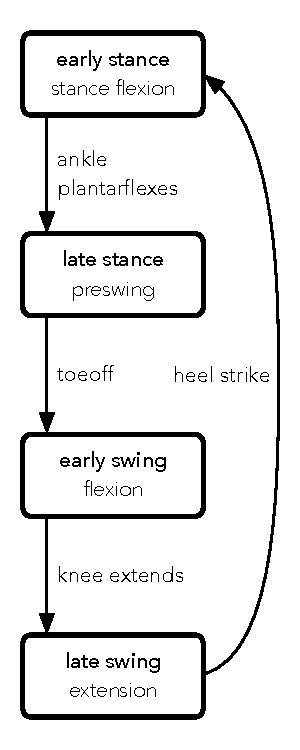
\includegraphics[width=\linewidth]{impedance_control_state_flow}
    \caption{Finite state machine used for the quasi-stiffness control proposed
    by \citet{sup2007design}. In each state the control employs impedance
    functions that determine the behavior of the ankle and knee joints of an
    active transfemoral prosthesis.}
    \label{fig:impedance_control_state_flow}
\end{marginfigure}
This strategy has been implemented on both transtibial \citep{shultz2014walking}
and transfemoral \citep{lawson2014robotic} active prostheses and has improved
amputee gait characteristics over those provided by passive prostheses.
Moreover, by tuning impedance parameters for specific tasks and augmenting the
finite state machine, researchers have extended impedance control to help
amputees to walk up and down slopes \citep{sup2011upslope} and stairs
\citep{lawson2013control}, run \citep{huff2012running, shultz2015running}, and
execute sit-to-stand motions \citep{varol2009powered}.  \citet{lenzi2014speed}
present a similar method, in which a look-up-table directly stores the
quasi-stiffness curve with respect to angle and velocity.  With this method,
\citeauthor{lenzi2014speed} obtain speed adaptation by linearly interpolating
between two look up tables representing slow and fast walking.

In contrast to the kinematic echo control strategy discussed earlier,
quasi-stiffness control should produce more reasonable interaction forces. This
is especially true when the prosthesis encounters an unexpected disturbance, as
the control does not try to follow a specific trajectory with high precision and
thus high feedback gains. However, whereas impedance control as originally
proposed by \citet{hogan1985impedance} advocated independent specification of
the disturbance response torque and the torque required to achieve the desired
motion, the quasi-stiffness control strategies we have discussed use the same
behavior for both. 

Recently, several research efforts have investigated dynamic control strategies
that provide both a feed forward element that generates the desired motion and a
feedback element that responds to disturbances. Such approaches allow one to
tune these these two aspects separately. While these approaches are
decentralized in that they do not require state information of the amputee, they
do borrow aspects of centralized approaches such as trajectory planning, and
model-based computation of feed-forward torques.

For example, \citet{lenzi2014speed, lenzi2014minimum} compute minimum jerk
trajectories for the knee and ankle joints during the swing phase. These
trajectories are parameterized by fifth order polynomials that connect the
initial states of the knee and ankle joints, measured just before toe-off, to to
the desired final states, specified for both joints as zero angle, velocity, and
acceleration. The ankle joint uses a single trajectory, while the knee joint
uses two trajectories, one that connects the initial state to a maximum knee
flexion state and one that connects the maximum knee flexion state to the final
state.  Using a model of the system represented by Euler-Lagrange dynamics
equations (\cref{eq:euler_lagrange}) one can calculate the required feed forward
torque to follow the planned trajectories. Minimizing the jerk, the derivative
of acceleration, helps ensure smoothness of the computed torques. A proportional
derivative feedback control then determines the disturbance response behavior.
The use of a strong feed forward term allows for lower PD feedback gains and
more compliant behavior.

A disadvantage of the minimum jerk trajectory approach is it generates and
executes a trajectory whose duration is heuristically determined at toe-off.
Recently, \citet{gregg2014virtual, zhao2016first} have proposed methods similar
to the centralized virtual constraint control discussed in
\cref{sec:back_centralized_control}, in which the natural progression of a phase
variable determines the rate at which the control follows preplanned
trajectories. \citet{gregg2014virtual} chooses to follow the ankle-foot and
knee-ankle-foot rollover shapes, which are defined as the location of the center
of pressure with respect to coordinate systems attached to the shank and the
ankle-hip line respectively. The center-of-pressure naturally becomes the phase
variable for these trajectories. The observation that the roll-over shapes are
invariant across walking speed, shoe geometry, and amputee weight motivates this
choice. In this strategy, a model-based feedback linearization controller
enforces adherence to these desired trajectories as the center of pressure
progress through its natural dynamics. This formulation provides both the feed
forward torque command and a disturbance response command that provides
exponential converge to the desired rollover shapes. 

As we noted earlier for centralized robotic control approaches, a downside of
these two trajectory following controllers is their reliance on accurate
dynamics models to compute feed forward torques. To overcome this issue,
\citet{zhao2016first} propose a model-independent virtual constraint control. In
this scheme, quasi-stiffness control provides a feed-forward torque signal that
reduces the dependence on the model. A quadratic program then computes the
minimum required extra effort to ensure convergence to a preplanned trajectory
that is parameterized with respect to hip angle.

\section{Bioinspired Control for
Prostheses}\label{sec:back_bioinspired_pros_control} 

The dynamic control prosthesis control strategies we outlined in the previous
section in some sense all provide a feed-forward torque that generates a desired
nominal trajectory, and an impedance behavior that determines the disturbance
response characteristics. In the case of quasi-stiffness control, the same
function encodes both of these characteristics.  In the case of trajectory
following controllers, model inversion provides the necessary torque to execute
the plan while either a proportional derivative controller, feedback
linearization, or control Lyapunov function provides impedance behavior.
However, it is not clear that these approaches generate the impedance responses
of the system we actually want to replicate in the field of prosthetics, that of
the amputee's missing limb. In the biological leg, impedance characteristics may
play a crucial role when it comes to stabilizing movement
\citep{won1995stability, burdet2001central} and changes in response to a number
of factors including any of mean ankle torque, ankle position, perturbation
amplitude, and muscle fatigue \citep{kearney1989system}.

An alternative approach to developing prosthesis control, which may better model
joint quasi-stiffness and joint impedance, is to model the underlying biological
neuromuscular dynamical system that gives rise to these characteristics. Two
hypothesized mechanisms that govern the neuromuscular system are central pattern
generators (\cref{sec:back_CPG}) and reflexes
(\cref{sec:back_neuromuscular_reflexes}). These two mechanisms are naturally
decentralized and dynamic and are thus attractive models to utilize in a
prosthesis controller.

\subsection{Central Pattern Generators}\label{sec:back_CPG}
\subsubsection{Central Pattern Generators in Biology}
\emph{Central Pattern Generators} (CPGs) are hypothesized nonlinear
oscillators, comprised of neurons in the central nervous system, that can
autonomously generate periodic neural activation
patterns~\citep{ijspeert2008central}.  \citet{brown1911intrinsic} first
suggested their existence based on experiments he conducted on decerebrated and
deafferented cats. In these experiments, \citeauthor{brown1911intrinsic} severed
both the afferent pathways (that carry sensory information) and efferent
pathways (that transmit higher level commands from the brain to motor neurons).
Despite the lack of high level control and sensory feedback, the cats still
displayed cyclical motions in their hind legs similar to those seen during
normal gait. This result suggests CPGs may play an important role in generating
locomotion controls in vertebrate animals. Similar cyclical neural activity
(called fictive locomotion) has been found in isolated lamprey spinal cords
\citep{cohen1980neuronal}, salamanders \citep{delvolve1999fictive}, and frog
embryos \citep{soffe1982tonic}. 

\begin{marginfigure}
    \centering
    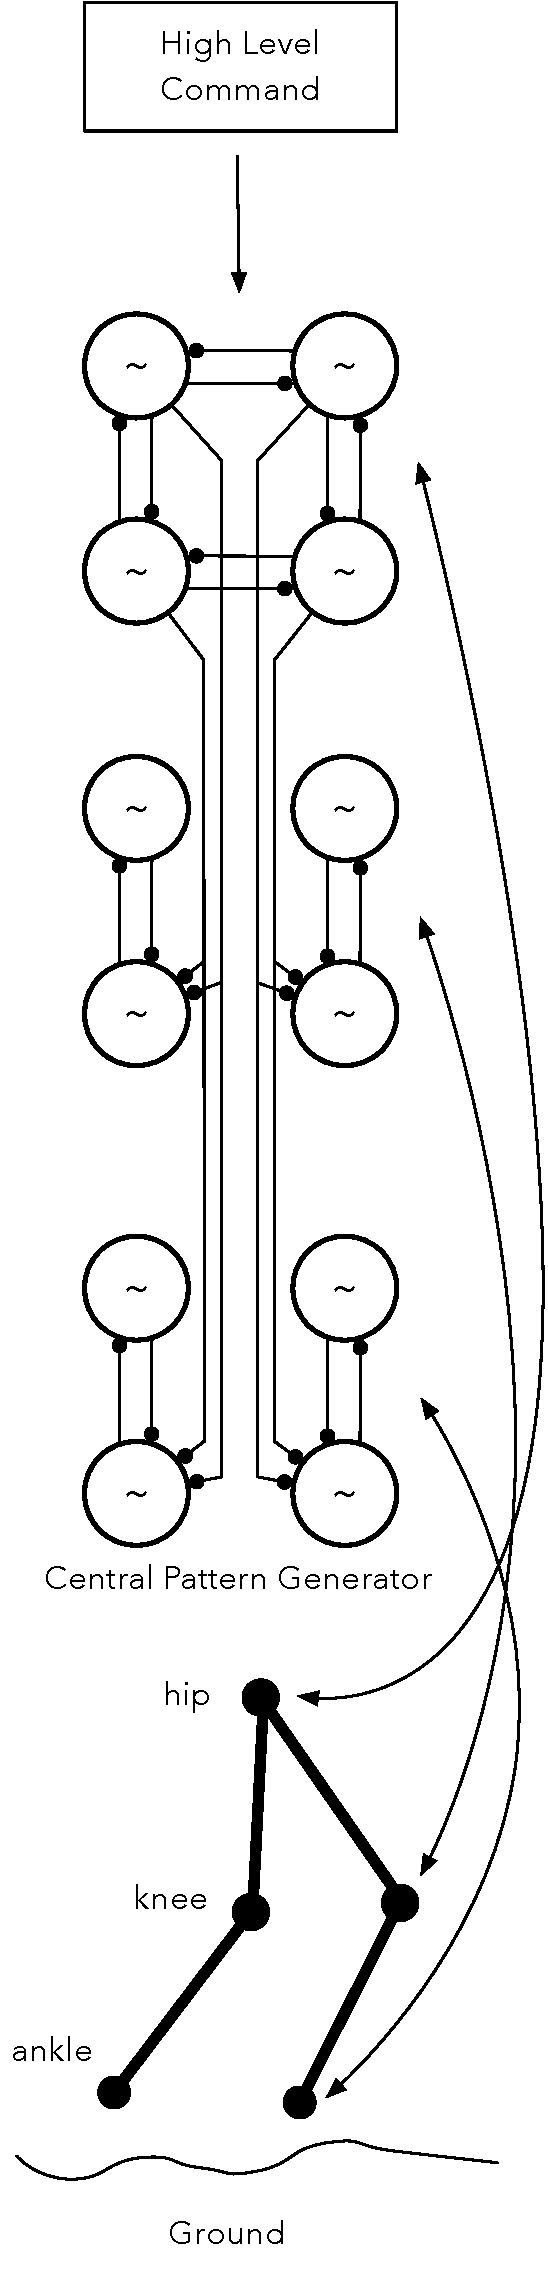
\includegraphics[height=6.25in]{CPG_diagram}
    \caption{Central Pattern Generator for bipedal locomotion as described in
    \citet{taga1991self}. Six neural oscillators receive feedback from and
    command joint torques for the hips, knees, and ankles of a planar biped
    model. A one dimensional high-level control signal enables control of speed
    and elicits gait transitions.}
    \label{fig:cpg_diagram}
\end{marginfigure}
Moreover, research has shown that stimulation of a region of the brain stem
called the Mesencephalic Locomotor Region (MLR) can manipulate the neural
activity generated by CPGs. For example, electrical stimulation of the MLR led
to gait transitions in both decerebrated cats \citep{shik1966control} and
salamanders \citep{cabelguen2003bimodal}.  Therefore, CPGs may serve as a form
of dimensionality reduction and decentralization for the biological control
system as low-dimensional, high-level signals from brain can shape the
high-dimensional, low-level CPG output. Consequently, CPGs may also represent
an attractive option for robotic legged locomotion controllers as
decentralization and dimensionality reduction are desirable properties in this
domain as well.

\subsubsection{Neuromechanical Models with CPGs}
The seminal work on CPG-based bipedal locomotion control is presented in
\citet{taga1991self}. In this model, a CPG neural network of six interconnected
oscillators describes the joint torques applied to a four link biped model.
Differential equations, first presented in \citet{matsuoka1987mechanisms} with
additional sensory feedback from joint and inertial link angles, describe the
output of the CPG network. The resulting biped model walks with a natural gait
featuring both single and double support and demonstrates robustness to a
variety of disturbances including changes to ground stiffness, damping, and
slope. Additionally, tuning a single parameter induced a transition from walking
to running in the model in a manner comparable to the biological gait
transitions observed after stimulation of the MLR.

CPGs have successfully controlled several bipedal humanoid robots. For example,
\citet{endo2005experimental} used \citeauthor{matsuoka1987mechanisms}'s
nonlinear oscillators along with by bio-inspired feedback pathways that regulate
ground reaction forces and body roll to generate desired foot trajectories for
the bipedal QRIO robot. As in \citeauthor{taga1991self}'s simulations walking
speed can be controlled via adjustment of a single parameter and the robot is
robust to changes in step height. Authors have also successfully employed other
nonlinear oscillator models. In \citet{shan2002neural}, a Recurrent Neural
Network generates oscillatory signals for a 20-DOF humanoid robot, HOAP-1, that
allow it to walk up and down stairs. In \citet{righetti2006programmable},
programmable ``Hopf'' oscillators \citep{righetti2006dynamic} learn desired
walking trajectories through entrainment enabling HOAP-2, a 25-DOF robot, to
walk forwards and backwards at varying speeds and step lengths.  

\subsubsection{CPGs for Prosthesis Control}
CPGs have also been proposed for controlling both mechanically-passive and
active lower limb prostheses.  \citet{nandi2009development} optimize CPG
parameters to fit recorded knee angle trajectories from healthy human subjects.
During walking, the CPG entrains desired knee motions to the oscillations of the
amputee's hip joint. The desired knee angles are achieved in a
mechanically-passive prosthesis via online adjustment of the knee damping.
Similarly, \citet{torrealba2010through, mora2012cybernetic} also use a CPG to
control a mechanically-passive variable damping prosthesis but use phase
resetting to synchronize the amputee and CPG dynamics. 

For active prostheses, \citet{geng2012design} suggest using a Hopf oscillators
to fit the trajectory of the knee angle during walking. \citet{guo2010study}
extend the idea of using a CPG for active prosthesis control by proposing a
hierarchical approach with a support vector machine (SVM) at the high-level
inferring amputee intent from EMG signals, and a CPG at the lower-level
determining the desired knee and ankle angles for an active transfemoral
prosthesis. However, in both cases, the authors do not provide experimental
results on real prosthesis hardware. Moreover, unlike in
\citeauthor{taga1991self}'s original work, these proposed CPG networks for
prostheses generate desired joint kinematics instead of torques. Consequently,
these controllers may not allow prostheses to exhibit the dynamism and
compliance we desire.

\subsection{Neuromuscular Reflexes}\label{sec:back_neuromuscular_reflexes}
\subsubsection{Neuromuscular Reflexes in biology}
Around the same time \citeauthor{brown1911intrinsic} hypothesized the existence
of central pattern generators, \citet{sherrington1910integrative,
sherrington1910flexion} suggested another mechanism for oscillatory neural
signals: chains of \emph{reflexes}, or local feedback loops, that trigger in
response and entrain to sensory signals. \citeauthor{sherrington1910integrative}
identified complex, multi-joint, multi-limb reflex arcs involving both
excitation and inhibition in response to cutaneous stimulation in decerebrated
cats. Moreover, he observed rhythmic stepping behavior in decerebrated cats
suspended off the ground and concluded that the behavior emerged reflexively
based on proprioceptive signals emanating from the muscles themselves and not
from centrally generated oscillatory signals.

In animal experiments discussed earlier, while CPGs can go a long way towards
explaining locomotion neural activity, they still do not fully explain all
observed phenomena. Reflexes likely at least shape locomotion activation
patterns through entrainment, for example in Lamprey's movement of the tail
generates activation in the spinal chord of equal frequency
\citep{mcclellan1993mechanosensory}, and phase resetting, as demonstrated by the
ability of decerebrated cats to walk on treadmills across a range of speeds
\citep{rossignol2000locomotion}.

For human and primate bipedal locomotion, the role of CPGs is more muddied and
the role of reflexes more evident than for decerebrated cats and simpler
vertebrate animals \citep{mackay2002central, vaughan2003theories,
nielsen2003we}. This is perhaps due to the demands of controlling the inherently
unstable dynamics of upright walking \citep{capaday2002special}. For example,
while rhythmic spinal activity has been observed in humans, it is not clear if
the neural signals are an example of autonomous fictive motion, indicative of a
CPG, or entrainment with stretch reflexes in leg muscles
\citep{capaday2002special, stewart1991modulation}. In this case, we can also
look to robotics to provide insight about biology: in the previously discussed
experiments on humanoid robots controlled by CPGs, a significant reduction in
robustness was observed after blocking sensory feedback pathways
\citep{endo2005experimental, righetti2006programmable} indicating CPGs alone may
not fully explain bipedal locomotion. Whereas research has not yet clearly
established the presence of a CPG driving human locomotion, research has
identified many reflexes that contribute to locomotion such as the Hoffman
reflex (H-reflex) of the soleus ankle plantarflexor muscle
\citep{capaday1987difference}, stretch reflex in the soleus
\citep{yang1991contribution}, soleus force feedback \citep{grey2007positive},
and cutaneous reflexes that induce withdrawal responses \citep{yang1990phase}. 

\subsubsection{Neuromuscular Models with Reflexes}
To model the potential interplay between muscular reflexes and CPGs in human
locomotion \citet{ogihara2001generation} extend the model presented in
\citet{taga1991self} by adding muscles stimulated by alpha motor neurons. This
model simulates nine muscles of the leg, each stimulated by an alpha motor
neuron that receives input from a CPG oscillator and proprioceptive feedback
from one or more muscles. The muscles produce forces according to their state
and activation input (computed using models presented in
\citet{pierrynowski1985physiological} and \citet{davy1987dynamic}). These forces
are applied to constant moment arms in order to produce joint torques summed
about joints as in a virtual model control. The authors optimize the cost of
transport of transport of the biped with a genetic algorithm and achieve a gait
with human-like kinematics and kinetics. Moreover, the forces produced by many
of the muscles resemble those produced during human locomotion. Despite the fact
that the CPG used in this model received no feedback signals, the resultant gait
still exhibited a small degree of robustness to perturbations although not as
much as \citeauthor{taga1991self}'s model. The author's attribute the robustness
to the stabilizing feedback provided by muscle reflexes. 
\begin{marginfigure}
    \centering
    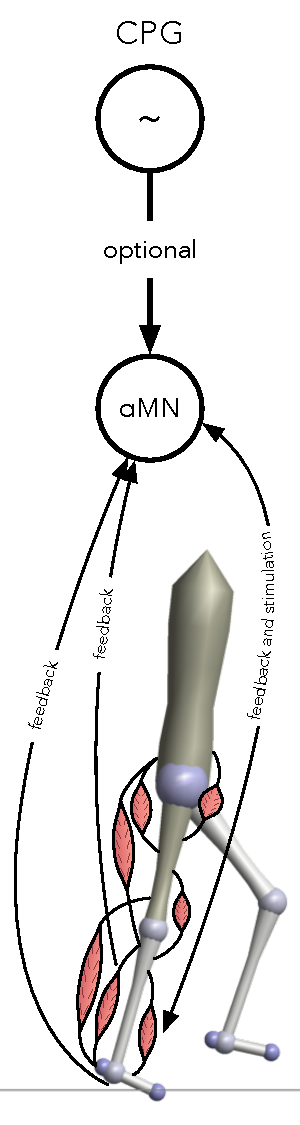
\includegraphics[height=5.5in]{reflex_diagram} 
    \caption{Neuromuscular models with reflex feedbacks. The model developed by
    \citet{ogihara2001generation} activates individual muscles according to the
    activity of a CPG and proprioceptive reflexes that can involve the muscle
    itself, other muscles, and ground contact sensing.  \citet{geyer2010muscle}
    does away with the CPG and achieves locomotion with only reflex feedbacks.}
    \label{fig:reflex_diagram}
\end{marginfigure}

Whereas models and robot experiments show reflexes are vital for maintaining
bipedal gait stability, the same cannot be said about CPGs. In fact, as shown by
\citet{geyer2010muscle}, it is possible to simulate robust and human-like
bipedal locomotion using only reflexes. This work employs a neuromuscular
model, similar to that used in \citet{ogihara2001generation}, but does away with
the feed forward CPG stimulations sent to alpha motor neurons. Instead,
\citeauthor{geyer2010muscle} hypothesize the existence of several force and
length muscle reflexes that implement three key aspects of bipedal locomotion:
compliant leg behavior, preventing joint over extension, and providing trunk
stabilization. The gait achieved by this model is more robust than and more
accurately reproduces kinematics, kinetics, and ground reaction forces seen in
human walking than \citeauthor{ogihara2001generation}'s model. Moreover, it also
produces human-like stimulations for many of its muscles.

While we cannot say based on this result alone that CPGs do not play an
important role in human locomotion, the fact that human locomotion can emerge
from purely reflexive controls increases the attractiveness of using this
approach for prosthesis control. The reflex-only paradigm may be easier to
design and optimize than the CPG+reflex paradigm for two reasons: First, the
reflex connection graph used by \citet{geyer2010muscle}'s reflex-only model is
much more sparse than that used by \citet{ogihara2001generation} CPG+reflex
model. Using a sparse set of reflexes and no CPG reduces the number of
parameters that we must tune in order to achieve locomotion. Second, the
reflexes in the reflex-only model are functionally motivated, which may increase
our intuition about the role of each reflex and assist our ability to tune the
model's parameters. This is evidenced by the fact that
\citeauthor{geyer2010muscle} hand tuned the parameters of their model whereas
\citeauthor{ogihara2001generation} used a genetic algorithm.  Moreover,
functionally motivated feedbacks used in the reflex-only approach has allowed
further research to extend this model to include swing leg placement
\citep{desai2013muscle}, 3D locomotion, running, speed changes, stair and slope
negotiation, turning, and obstacle avoidance \citep{song2015neural}.  

The robustness properties exhibited by neuromuscular model are especially
relevant to our goal of developing a robust prosthesis control that will help
transfemoral amputees avoid falls. In \citet{song2015neural} the author's
improve the model's robustness by incorporating reflexes that place the swing
leg into target landing angles. The authors optimize this model to achieve a
combination of robustness and energy efficiency.  The resulting gait can walk on
terrains featuring random steps up to $\unit[\pm 6]{cm}$ (50 \% success rate)
and rejects pushes in both the forward and backward directions at various points
in the gait cycle. In another work, \citet{murai2011neuromuscular} subject a
neuromuscular model, initially trained to match kinematic data of single
subject, to impacts during early and late swing. They find the learned model
exhibits the elevating and lowering trip response strategies of the biological
leg despite not being explicitly trained to do so. These disturbance response
characteristics point to reflex control providing the appropriate quasi-static
and impedance behaviors.

\subsubsection{Neuromuscular Reflexes for Prosthesis Control}
\begin{marginfigure}
    \centering
    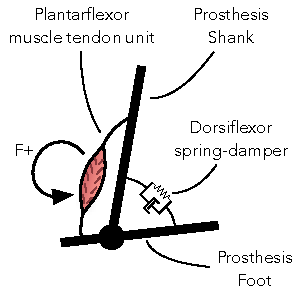
\includegraphics[width=\linewidth]{eilenberg_diagram} \caption{Neuromuscular
    model used by \citet{eilenberg2010control} to control an active ankle
    prosthesis. During stance, a virtual muscle driven by positive force
    feedback, generates plantarflexion torque. During swing, a virtual spring
    damper provides dorsiflexion torque to prevent toe scuffing.}
    \label{fig:eilenberg_diagram}
\end{marginfigure}
Motivated by the robustness and natural gait achievable by neuromuscular
reflex control, past research has applied this model to active prostheses and
exoskeletons. \citet{eilenberg2010control} applied a simplified version of the
control to a powered ankle prosthesis (\cref{fig:eilenberg_diagram}). In this
work, the neuromuscular model was reduced to a single ankle plantarflexor muscle
driven by a positive force feedback reflex during stance. During swing, the
control applies torque to dorsiflex the ankle according to a virtual spring
damper model. In amputee testing of a prosthesis controlled by the neuromuscular
model the control produced ankle kinematics and kinetics similar to those
observed in healthy human walking. Significantly,
\citeauthor{eilenberg2010control} found evidence that the robustness and
entrainment properties observed in neuromuscular model simulations may carry
over to amputee gait as well. The author's note that the prosthesis
automatically adapts torque output when walking on slopes, producing more
plantarflexion torque when walking up slopes and less when walking down slopes.
Additionally, \citet{markowitz2011speed} found that a similar neuromuscular
reflex model automatically produced more ankle plantarflexion work as the
amputee increased his gait speed.

\subsubsection{EMG-based Control}\label{sec:back_emg_control}
The inclusion of user intent recognition via surface electromyography (EMG)
signals represents an interesting extension of neuromuscular reflex prosthesis
control. In these approaches, muscle activity in the residual limb is directly
measured via EMG sensors embedded in the amputee's prosthesis socket. These EMG
sensors are then used to control the torque generation of the amputee's leg
prosthesis. Because neuromuscular models describe how joint torque is generated
in response to muscle activations, a natural approach is to use the EMG signal
in reflex pathways in order to activate virtual muscles. This is the approach
proposed by \citet{wu2011electromyography}. In this work,
\citeauthor{wu2011electromyography} control an active transfemoral prosthesis
using EMG sensor readings from the residual thigh to activate virtual knee
flexor and extensor muscles according to a linearised Hill muscle model. The
resulting prosthesis control allowed an intact subject wearing the prosthesis
via an able-bodied emulator to achieve nearly normal gait. In a similar
approach, \citet{wang2013proportional} use EMG signals to modify the gain on a
positive torque feedback loop (similar to positive force feedback used in
\citet{geyer2010muscle}) in order to control ankle plantarflexion torque. As
seen in healthy human walking, toe off angle and ankle net work increased with
increasing walking speed.

These two works have demonstrated that neuromuscular approaches have enabled EMG
based control to go beyond its typical application of high-level mode
recognition. For example, \citet{huang2009strategy, huang2011continuous}, and
\citet{hargrove2015intuitive} recognize walking modes, such as level ground
walking, ramp and stair ascent, and ramp and stair descent, by training
classifiers on features of EMG and mechanical sensor data. In contrast, the EMG
+ neuromuscular approaches allow the use typically noisy EMG sensor data for
low-level continuous control. \citet{wu2011electromyography} and
\citet{wang2013proportional} propose that because EMG + neuromuscular approaches
model physiologically plausible feedback loops and dynamics, they may allow
amputees to use muscle activations to control their prostheses in an intuitive
way.

\subsection{Conclusion} 
In summary, simulations and implementations of the neuromuscular reflex control
approach have repeatedly demonstrated its ability to generalize to a variety of
situations and exhibit robustness to a variety of disturbances. Due to the gait
deficits and fall risk transfemoral amputees face, these two properties make
this control paradigm very attractive for application to transfemoral prostheses
. Moreover, neuromuscular approaches have been successfully extended with EMG
sensor feedback from amputees' residual limbs, enabling intuitive low-level
prosthesis control. In contrast, other control approaches for prostheses such as
quasi-stiffness control have not demonstrated these properties. Importantly,
neuromuscular control addresses \cref{chal:dynamic,chal:incomplete_state} of
amputee locomotion~(\cref{sec:intro_challenges}) as we can implement them via a
decentralized, sparse set of reflexes and they allow for dynamism by providing
both a quasi-stiffness and impedance response via the dynamics of the
stimulated muscle models..

As yet, there have not been any published works applying neuromuscular reflex
control to active knee and ankle transfemoral prostheses. Therefore, in this
thesis, we work towards this goal with the hope of improving transfemoral
amputee gait robustness and naturalness. \Cref{sec:neuro_model} will review the
details of the particular neuromuscular implementation used in this thesis.

\section{Prosthesis Design}\label{sec:back_pros_design}
We can trace efforts to build an active knee-ankle prostheses to the seventies
when \citet{flowers1974use} created an active knee-ankle prosthesis emulator in
order simulate potential control schemes. This prosthesis used a hydraulic
actuator capable of producing $\unit[90]{N \cdot m}$ of torque and
$\unitfrac[0.5]{rev}{s}$ of no-load speed, sufficient for simulation of passive
prostheses. With this device, \citet{donath1974proportional} tested proportional
EMG control, a problem researchers are still investigating today
(see~\cref{sec:back_emg_control}). Indeed, this line of research proved to be
far ahead of its time, as most relevant research in active lower-limb prostheses
design has occurred only in the last ten years. The recent interest in active
knee ankle prostheses has been spurred by hardware improvements that allow
designs to approach the strength, speed, and low weight of the biological leg.
Enabling technologies include power-dense brushless motors, motor controllers,
and lithium-ion batteries, inexpensive microcontrollers and inertial measurement
units (IMUs), and strong but light composite materials such as carbon fiber.
With these advancements, engineers have successfully designed prostheses to meet
or exceed the requirements for walking~(\cref{tab:walking_requirements}).
\begin{margintable}
  \centering
  \begin{tabular}{lll}
    \toprule
    & Ankle Max & Knee Max \\
    \midrule
    Velocity & \unitfrac[0.72]{rev}{s} & \unitfrac[1.17]{rev}{s}\\
    Torque & $\unit[130]{N \cdot m}$ & $\unit[57]{N \cdot m}$\\
    Power & \unit[350]{W} & \unit[120]{W}\\
    \bottomrule
  \end{tabular}
  \caption{Required knee and ankle torque, velocity, and power for walking
  (\unitfrac[1.40]{m}{s} average speed, scaled to \unit[85]{kg} subject,
  data from \citet{winter2009biomechanics})}
  \label{tab:walking_requirements}
\end{margintable}

In this \namecref{sec:back_pros_design}, we review a number of recent prosthesis
designs and analyze their ability to enable dynamic locomotion
(\cref{chal:dynamic,chal:incomplete_state} of transfemoral prosthesis locomotion).  To address
this challenge, prostheses should be able to regulate their output joint torques
and behave as though they have inertial properties similar to that of a normal
human leg. This will ensure that the prosthesis will emulate the energy
efficient gaits of normal walking and remain compliant to unforeseen
disturbances and uneven terrain.

\subsection{Direct Drive Transfemoral Prostheses}\label{sec:back_direct_drive}
\begin{marginfigure}
    \centering
	\begin{subfigure}[t]{\linewidth}
    	\centering
        %\includegraphics{}
        \missingfigure{Gen 1}
        \caption{Generation 1 used ball screw transmissions, \unit[200]{W}
        brushless motors, and a unidirectional parallel spring in the ankle that
        reduced motor torque requirements \citep{sup2009preliminary}.}
        \label{fig:vanderbilt_gen_1}
	\end{subfigure}

	\begin{subfigure}[t]{\linewidth}
    	\centering
        %\includegraphics{}
        \missingfigure{Gen 2}
        \caption{Generation 2 replaced ball screws with custom gear-based
        transmission that is less noisy and more durable
        \citep{lawson2013control}.}
        \label{fig:vanderbilt_gen_2}
	\end{subfigure}

	\begin{subfigure}[t]{\linewidth}
    	\centering
        %\includegraphics{}
        \missingfigure{Gen 3}
        \caption{Generation 3 features a modular design with separable knee and
        ankle units \citep{lawson2014robotic}.}
        \label{fig:vanderbilt_gen_3}
	\end{subfigure}
    \caption{Vanderbilt University's Robotic Transfemoral Prostheses.}
    \label{fig:vanderbilt_prostheses}
\end{marginfigure}

The most common approach for active transfemoral prosthesis design employs
electric motors, coupled to transmissions, that directly drive the knee and
ankle joints. The transmissions may utilize a combination of gears, chains,
belts, ball screws, and four-bar-mechanisms in order to increase the torque
output of the actuator, at the expense of speed, in order to satisfy the
requirements listed in \cref{tab:walking_requirements}. A successful line of
transfemoral prostheses following this design paradigm comes from Vanderbilt
university. The first prosthesis in this line \cref{fig:vanderbilt_prostheses}a
used a pair of ball screw transmissions and brushless motors capable of
\unit[200]{W} of continuous power output to drive its knee and ankle joints
\citep{sup2009preliminary}. 

With these actuators, the knee motor can achieve the required peak torque and
peak power intermittently (\cref{tab:walking_requirements}). However, the ankle
motor may be overly stressed due to the high requirements of walking. To remedy
this, this prosthesis includes of a unidirectional parallel spring in the ankle
that reduces the required ankle motor torque. As shown in figure
\cref{fig:ankle_torque_vs_angle}, during level ground walking, a linear torsion
spring accounts for a significant portion of the ankle's torque versus angle
relationship. Therefore, incorporating a spring into the ankle offloads this
portion of the torque from the motor. The ankle motor only needs to provide the
delta between the desired output torque and the linear spring. As a result, the
spring reduces motor energy consumption, heat generation, and transmission wear.

Further improvements resulted in two more generations of prostheses
(\cref{fig:vanderbilt_gen_2,fig:vanderbilt_gen_3}) \citep{lawson2013control,
lawson2014robotic}. These versions replaced ball screw transmissions with
a multi-stage belt/chain due to the improved packaging and reduced noise and
wear they afford (Michael Goldfarb, personal communication, September 18, 2013).
With these prostheses, researchers have extensively tested a variety of control
strategies including quasi-stiffness control \citep{sup2009preliminary,
sup2011upslope, lawson2013control, lawson2014robotic, lenzi2014speed}, EMG-based control
\citep{ha2011volitional, varol2010multiclass}, minimum jerk trajectory following
\citep{lenzi2014minimum}, and virtual constraint control
\citep{gregg2014virtual}. 

Additional prostheses in the direct drive category include AMPRO
\citep{zhao2016first}, and a commercially available active knee and ankle
prostheses: the Össur Power Knee and Proprio Foot. The AMPRO prosthesis features
two 374 W motors coupled to Harmonic Drive transmissions.
\citet{zhao2016first}, use this prosthesis to asses the merits of a virtual
constraint controller. The Össur Power Knee features an electric motor that can
provide torque to facilitate sit-to-stand motions, stair climbing, and active
extension and flexion during walking. The Proprio Foot also features electric
actuation that allows it to adapt to terrain and dorsiflex the ankle during
swing to help avoid trips. 
\begin{marginfigure}
    \centering
    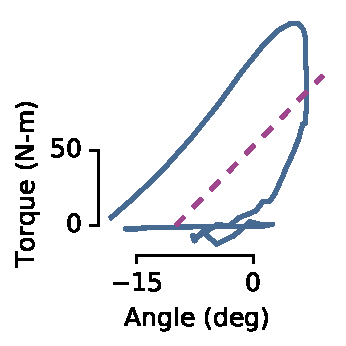
\includegraphics[width=\linewidth]{ankle_torque_vs_angle}
    \caption{Torque vs angle relationship for the ankle during level ground
    walking. A linear spring relationship captures a significant portion of
    ankle function during stance. Data from \citet{winter2009biomechanics}
    scaled to 85 kg subject.}
    \label{fig:ankle_torque_vs_angle}
\end{marginfigure}


\subsubsection{Torque Control Strategies for Direct Drive Prostheses}
In order to achieve dynamic locomotion capabilities, it is crucial that
prosthesis designs allow for closed loop control of torques. To do this control
system must be able to accurately measure the torque at the joint output. There
are two main strategies for torque measurement used by direct drive prostheses.

The first strategy is to measure the current draw of the motors windings, which
is related linearly to the motor torque. One can then multiply this measurement
by the gear ratio to obtain an estimate of the output joint torque. This is the
method used by Generations 2 and 3 of the Vanderbilt prosthesis as well as the
AMPRO prosthesis. The benefit of this method is that it utilizes existing
hardware and allows one to use high frequency current control modes of motor
drivers. However, a drawback of this method is that it measures the torque
before the transmission. Consequently, it does not account for frictional
losses, which can be difficult to model, especially for geared systems. A
strategy that deals with this problem is to install load cells in series with
the motor after the transmission, as was done on Generation 1 of the Vanderbilt
prosthesis. With this method, the closed-loop control can compensate for
frictional losses as they are included in the torque measurement. 

However, this method may still not address a second problem: sluggish passive
dynamics caused by reflected inertia and damping. Reflected inertia refers to
the apparent magnification of motor rotor and gearing inertia on the outside of
gearbox.  We can derive this effect through Newton's second law for the geared
motor
\begin{align}
    J_i \ddot{\theta}_i = \tau_i - b_i \dot{\theta}_i.
\end{align}
Here, $\theta$ and its derivatives refer to angular states of the motor, $b$
is the damping constant, $J$ is the inertia and $\tau$ is the motor torque. We
use subscript $i$ to refer to these quantities as seen before the gear
reduction, and subscript $o$ to refer to those quantities reflected outside of
the motor. Plugging in $\theta_i = n \theta_o$ and $\tau_i = \frac{1}{n}
\tau_o$, where $n$ is the gear ratio, and multiplying through by $n$ yields
\begin{align}
    J_i n^2 \ddot{\theta}_o &= \tau_o - b_i n^2 \dot{\theta}_o \\
    \implies \quad J_o \ddot{\theta}_o &= \tau_o - b_o \dot{\theta}_o.
\end{align}
These equations show that the inertia and damping of the motor rotor are
amplified by the square of the gear ratio. As prostheses may often use gear
ratios in excess of 100:1, this effect can be substantial. 

\begin{table}
  \centering
  \begin{tabular}{lll}
    \toprule
    & Knee & Ankle \\
    \midrule
    rotor inertia & $\unit[0.035]{kg \cdot cm^2}$ 
        & $\unit[1.210]{kg \cdot cm^2}$\\
    gear ratio & 176:1 & 115:1 \\
    reflected inertia & $\unit[0.11]{kg \cdot m^2}$ & 
        $\unit[1.6]{kg \cdot m^2}$\\
    human inertia & $\unit[0.66]{kg \cdot m^2}$  & $\unit[0.019]{kg \cdot m^2}$\\
    percent increase & 17\% & 8400\% \\
    \bottomrule
  \end{tabular}
  \caption{Estimated reflected inertia at knee and ankle joints of Generation 3
  Vanderbilt Prosthesis \citep{lawson2014robotic}. Motor data taken from Maxon
  Motors Catalog\citep{maxon_flat_motor,
  maxon_ec4pole} Knee reflected inertia compared to inertia of human shank and
  foot about knee. Ankle inertia compared to human foot about its center of
  mass. Human inertias estimated from \citet{winter2009biomechanics} for an
  \unit[85]{kg}, \unit[1.7]{m} tall person.}
  \label{tab:vanderbilt_reflec_interita}
\end{table}

For example, \cref{tab:vanderbilt_reflec_interita} shows the calculated
reflected inertias of the Maxon Motors used in Generation 3 of the Vanderbilt
prosthesis and compares the values to the estimated inertia of the shank and
foot about the knee and the foot about its center of mass. We see that at the
knee, the reflected inertia is roughly 17\% of that of the human shank and foot.
In practice, this value is likely several times higher after including the
inertia of the encoder, bearings, and gearing. Consequently, we can estimate
that the reflected inertia may be on the order of the leg itself. At the ankle,
the reflected inertia of the rotor alone is several orders of magnitude more
than that of the foot and more than twice that of the shank and foot. When we
also consider reflected damping and friction, the dynamics of prosthesis system
may be significantly slower than assumed.

The increase in joint impedance created by transmissions could present an issue
when attempting to execute dynamic behaviors involving impact such as running or
trip recovery. In an impact event, the impulse will move through the system at
the speed of sound through metal, roughly \unitfrac[6420]{m}{s} for aluminum
\citep{lide2004crc}. If the prosthesis is \unit[0.5]{m} long, the shock will
traverse its length in \unit[0.00008]{seconds}. This is about 10 times faster
than the typical \unit[1000]{Hz} control frequency of prosthesis control
systems, rendering closed loop torque control with load cells unresponsive. The
impact shock could cause damage to gearing and discomfort for the amputee.

%Reflected Inertia
%Vanderbilt gen 3 ankle = 1210 g*cm^2 * 115^2 in kg*m^2 = 1.6 kg*m^2
%Vanderbilt gen 3 knee = 35 g*cm^2 * 176^2 in kg*m^2 = 0.11 kg*m^2

%human leg for 1.7 85 kg = 0.6575 kg*m^2
%human foot for 1.7m 85 kg = 0.0187 kg*m^2

\subsection{Design of Dynamic Prostheses}
In contrast to the direct drive actuation discussed in the previous subsection,
prostheses that employ series elastic actuation may be better poised to achieve
dynamic locomotion \citep{pratt1995series}. This actuation scheme (illustrated
in \cref{fig:sea_diagram}) aims to solve the torque measurement and impedance
amplification caused by transmissions by placing a spring in series with the
actuator. Measuring the deflection of the spring allows for accurate closed-loop
control of the joint torque. Moreover, the spring low-pass filters external
impulses, granting the control system more time to move the motor rotor in
response to the external load.  Due to these properties, designers have
integrated series elastic actuators into a number of bipedal robots that seek to
achieve dynamic locomotion such as M2V2 \citep{pratt2008design} and ATRIAS
\citep{grimes2013atrias}.

\begin{marginfigure}
    \centering
    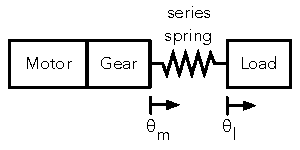
\includegraphics[height=6.25in]{sea_diagram}
    \caption{Series elastic actuation inserts a spring between the gear output
    and the load (here drawn as linear actuator for simplicity). Torque is
    measured via the spring deflection, $\tau = k(\theta_l - \theta_m -
    \theta_0)$ where $\tau$ is the output joint torque, $k$ is the spring
    constant, and $\theta_l$ and $\theta_m$ are the load and motor positions and
    $\theta_0$ is the spring's rest length.}
    \label{fig:sea_diagram}
\end{marginfigure}

Series elastic actuators have found use in a variety of transtibial and
transfemoral prostheses. We can further split these applications into two
categories, those that optimize the spring stiffness for control bandwidth
subject to shock tolerance and those that optimize spring stiffness to optimize
efficiency.

\subsubsection{Springs for Bandwidth and Shock Tolerance}
Adding a spring between the gear and load introduces additional dynamics between
external torques and torques applied to the gearbox as external torques must
physically displace the load before they generate torque on the motor. This
property can improve the shock tolerance of SEA actuators over that of direct
drive motors~\citep{robinson2000design}. However, by the same token, the SEA
also introduces additional dynamics between motor torque and load torque, hence
reducing force control bandwidth. Therefore, a trade-off exists between the
compliance of the actuator and speed with which it can generate desired torques.

\citet{au2007biomechanical, au2008powered} design powered ankle prostheses with
this trade off in mind. In these publications, the authors find that using an
SEA spring soft enough to protect the ball screw transmission results in
insufficient closed loop torque control bandwidth. To overcome this shortcoming,
the authors incorporate a parallel spring into the ankle as was done for some of
the knee and ankle prostheses discussed in \cref{sec:back_direct_drive}. Because
the parallel spring offsets the motor's torque requirements,
\citeauthor{au2008powered} find that it also improves the bandwidth of the
system from 4 Hz to 20 Hz, thereby exceeding the requirement for walking. 

\citet{caputo2013experimental} also used series elastic actuators in a robotic
prosthesis testbed. This system uses a large, \unit[1.61]{kW} offboard motor
connected to a light-weight prosthesis end-effector via a Bowden cable
transmission. The Bowden cable applies forces to one end of a fiberglass leaf
spring strain gauges measure its deflection. The author's note that the series 
springs isolate the prosthesis end effector from the motor's rotor inertia. With
this system the author achieve a large peak output torque ($\unit[175]{N \cdot m}$)
and high bandwidth (\unit[17]{Hz}), allowing them to rapidly test the effects of
different control strategies and emulate prosthesis hardware
\citep{caputo2015informing}.

\subsubsection{Springs for energy efficiency}
Designers can also tune series elasticity in order to improve energy efficiency
by mimicking the role of tendons in the biological human leg. In the human
ankle, the Achilles tendon, which is in series with the ankle plantarflexor
muscles, stores energy throughout stance and releases it just prior to toe-off,
producing a surge of mechanical power. During this process, the ankle
plantarflexor muscles hold the proximal end of the tendon nearly stationary via
isometric contraction. This kind of length-preserving muscle contraction
consumes relatively little metabolic energy compared to concentric or
length-shortening contractions \citep{rall1984energetic}. Consequently, ankle
elasticity helps store and release energy, thereby improving metabolic cost of
walking \citep{sawicki2009pays}.

Similarly, the SPARKy prosthesis uses a \emph{Robotic Tendon} comprised of
helical springs in series with the motor to store and release energy ankle
energy during stance \citep{hitt2007sparky, bellman2008sparky,
holgate2008sparky}. Adding a series spring changes the ankle motor movement to
that required to generate desired output torque given the stiffness of the
spring and trajectory of the ankle joint\sidenote{$\theta_m = \theta_l -
\nicefrac{\tau}{k} - \theta_0$, where $\tau$ is the desired ankle torque,
$\theta_l$ is the ankle trajectory, and $k$ and $\theta_0$ are the spring
stiffness and offset}. Therefore, with a properly tuned series spring the
design reduces motor movement and thus required motor power from \unit[250]{W}
to \unit[77]{W} \citep{hitt2007sparky}.

Transfemoral prosthesis designs have also sought to use springs in the knee
joint in order to improve energy efficiency. However, these prostheses require
more sophisticated designs due to the complex behavior of the knee. Whereas a
single spring relationship explains a significant portion of ankle joint
behavior (\cref{fig:ankle_torque_vs_angle}), as shown in
\cref{fig:knee_torque_vs_angle}, the knee joint requires two springs: one for
early stance and one for pre-swing and swing. Two prostheses that tackle this
design problem are AAAKP (agonist-antagonist active knee prosthesis)
\citep{martinez2008design, martinez2011antagonistic} and the CSEA (clutchable
series elastic actuator) knee \citep{rouse2014clutchable, rouse2015design}.

\begin{marginfigure}
    \centering
    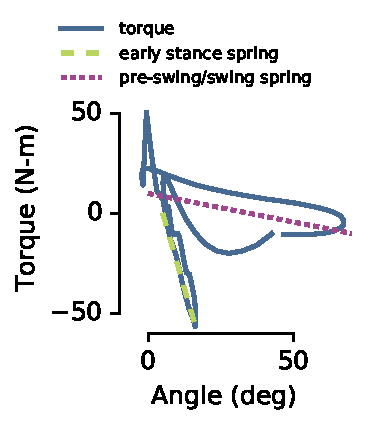
\includegraphics[width=\linewidth]{knee_torque_vs_angle}
    \caption{Torque vs angle relationship for the knee during level ground
    walking. Knee displays more complicated functionality than the ankle (see
    \cref{fig:ankle_torque_vs_angle}), with two distinct springs need to explain
    early stance and pre-swing/swing behavior. Data from
    \citet{winter2009biomechanics} scaled to 85 kg subject.}
    \label{fig:knee_torque_vs_angle}
\end{marginfigure}

The AAAKP prosthesis uses two unidirectional springs, one for extension and one
for flexion, each in series with its own actuator. With this setup,
AAAKP is able to store energy during the knee flexion phase just after heel
strike, and transfer it to a flexion spring for use during pre-swing and swing.
The prosthesis consumes just \unitfrac[5.6]{J}{stride}. However, the downside of
this design is inefficient use of actuator mass, as two electric motors are
required, one for extension and one for flexion.

A second concept is to use a series elastic actuator with a clutch on the motor
\citep{rouse2014clutchable, rouse2015design} The clutch saves energy by holding
the motor side of the series spring stationary while the spring is loaded in
early stance; no electrical energy is consumed holding the rotor in place. In
this design the spring-like behavior of the knee during swing is reproduced by
the electric motor alone unlike in the AAAKP prosthesis. Despite this, the
CSEA knee consumes less energy than the AAAKP, just \unitfrac[3.6]{J}{stride}.
Moreover, the simplified design of the CSEA has a mass of \unit[2.7]{kg} vs
\unit[3.6]{kg} for the AAAKP.

A potential drawback of SEA designs that are tuned for energy efficiency is that
they typically tune tune the spring stiffness to match observed quasi-stiffness
of the biological joint during a certain phase of the gait. However, this
stiffness value is not necessarily that which maximizes torque control
bandwidth. Therefore, while prostheses tuned for efficiency can consume less
energy, which is desirable for a product needing long battery life, they may
not represent the most versatile design for evaluating new control ideas or
different gait modes. 

\section{Stumble Recovery for Prostheses}\label{sec:back_stumble_recovery}
The prosthesis controls we reviewed in
\cref{sec:back_walking_review,sec:back_bioinspired_pros_control} primarily
sought to reproduce typical walking kinematics and dynamics. Some control
strategies, such as neuromuscular reflex control
(\cref{sec:back_neuromuscular_reflexes}) also demonstrated the ability to
generalize to sloped walking and changes in speed by producing more push off
work in these situations \citep{eilenberg2010control, markowitz2011speed}.
However, it is not clear that the low-level reflexes in the neuromuscular
control model will generate trip recovery responses, which in human control
likely utilize more complex supraspinal and cortical reflexes
\citep{eng1994strategies, schillings2000muscular, hofstad2009evidence}.
We therefore seek to improve upon neuromuscular control's inherent stability
by augmenting it with explicit trip detection and recovery actions.

As discussed in \cref{sec:intro_motivation}, falling and the fear of physical
activity it engenders are two major issues amputees face
\citep{miller2001prevalence}. Avoidance of physical activity can potentially
cause deterioration of strength, balance and control, which may lead to further
inactivity, debilitation, and social isolation. Currently, the microprocessor
controlled, mechanically-passive prostheses feature trip recovery modes
that ``lock'' or highly damp knee movement. However,
\citet{bellmann2010comparative} show that these modes fail to adequately respond
to trips during a large portion of swing due to knee buckling at touch-down.
Moreover, it is unclear that passive, locking responses are intuitive for
amputees or coordinate well with innate trip recovery responses, which can
require positive joint power \citep{cordero2005energy}. However, the advent of
active transfemoral prostheses give us the opportunity to replicate amputee's
preferred responses, which will hopefully yield more effective and intuitive
fall-prevention actions.

\subsection{Responses to Trips}

Able-bodied persons primarily use two strategies to recover from trips to their
swing legs: When the tripped in early swing, people usually use an
\emph{elevating strategy}, in which the knee is actively flexed to lift the foot
over and in front of the obstacle. In late swing, people typically use a
\emph{lowering strategy}, in which knee extensor muscles rapidly bring the foot
in contact with the ground in front of the obstacle \citep{eng1994strategies}.
In response to mid-swing trips, people may use either strategy
\citep{schillings2000muscular}. Finally, the \emph{delayed lowering} can also be
used in early swing. This strategy is an aborted attempt at an elevating
strategy, followed by a lowering strategy, and is used when the toe catches
on the obstacle \citep{eng1994strategies}.

Interestingly, \citet{shirota2015transfemoral} show that transfemoral amputees
using mechanically-passive prostheses utilize these same strategies despite the
lack of control and positive power production at the knee joint. Amputees
compensated for these deficiencies and achieved elevating, lowering, and delayed
lowering foot trajectories via movements of the hip and sound side leg. The lack
of sensory feedback information from the prosthesis leg to the nervous system
did not seem to impede utilization of these strategies.  Consequently, the
authors hypothesize that mimicking able-bodied responses to trips may also be
intuitive for amputee subjects. 

While amputees using mechanically-passive prostheses exploit the same strategies
as able-bodied subjects for trip recovery, they do not use these strategies in
the same proportions during the phases of swing as do able-bodied subjects.
Amputees typically use elevating strategies less frequently and lowering
strategies more frequently. This difference increases when the prosthesis is the
stance leg, and the intact leg is tripped. A possible reason for decreased
reliance on the elevating strategy may stem from the inability of
mechanically-passive prostheses to produce positive joint power.
\citet{cordero2005energy} show that in an elevating strategy, positive power is
required in the swing-leg's knee joint in order to rapidly flex the knee to
achieve obstacle clearance. Likewise, \citet{pijnappels2004contribution} show
that powered stance leg push-off helps raise the foot during the elevating
strategy. Empowering transfemoral prostheses with active joints may help
amputees more easily realize the elevating strategy, normalize amputee trip
recovery strategy selection, and allow them to recover from a larger range of
disturbances.

\subsection{Trip Detection and Classification}
Human responses to gait disturbances likely involve signal processing at the
supraspinal and cortical level. This is evidenced by the relatively high latency
($>\unit[100]{ms}$) of EMG signals relevant to the utilized strategy, the
utilization of both elevating and lowering strategies in mid-swing, the
existence of the delayed lowering strategy \citep{schillings2000muscular}, and
the inconsistent resolution of motor redundancy during the lowering strategy
\citep{eng1994strategies}. Furthermore, \citet{hofstad2009evidence} found that
latencies are further increased for amputee subjects executing obstacle
avoidance tasks, suggesting that amputee trip recovery may require additional
data processing and cognitive control as compared to able-bodied persons. 

A control system that seeks to be intuitive and effective for amputees by
mimicking their responses to trips needs to be able to model these complexities.
As a result, researchers have relied on data-driven and machine learning
approaches to detect and classify trips so that prostheses can take the
appropriate actions. All systems designed to date use a two-layer classification
scheme, where the first layer distinguishes trips from normal walking, and the
second layer classifies the recovery strategy as either elevating or lowering.
The first such system by \citet{lawson2010stumble} used Fast Fourier Transform
features of data collected from six accelerometers placed on the lower limb. To
collect training data, the author's outfitted healthy subjects with sensors, and
randomly subjected them to trips. They classified stumbles from normal walking
via a threshold on power between 10 and \unit[40]{Hz} and classified elevating
versus lowering strategies based on the root-mean-squared thigh acceleration in
a \unit[50]{ms} window before the stumble. \citet{zhang2011towards} further add
EMG sensors to the trip detection system, and employ outlier detection methods
so that the trips were not required in the training dataset. They find EMG sensors
improve the false alarm rate, at the expense of classification latency. However,
the false alarm rate is still quite high, corresponding to an incorrect positive
classification every \unit[1.6]{min}. Finally, \citet{shirota2014recovery} use
linear discriminant analysis on kinematic features from the tripped leg. They
find evidence supporting the use of the two-stage classification scheme, and
identify the optimal update frequency and length for the window in which they
compute features.

A major drawback of these previous works is that they report error rates based
on offline validation results; \ie they collect data from subjects who are
responding to trips and then evaluate how well the classifier would have
performed on the collected data. This is fundamentally different than online
validation, in which one reports the error rate obtained when using the
learned classifier to control the system. Previous work on a classifier for
recognizing gait modes such as level walking and stair and ramp ascent and
descent found that online error rates were significantly higher than offline
error rates \citep{hargrove2015intuitive}. As we discuss in
\cref{sec:proposed_trip_recovery}, it is likely this trend will hold true for
stumble classification as well.
